\begin{enunciado}
 En el plano af\'{\i}n y usando coordenadas cartesianas $xy$
 se consideran dos puntos
 $P_1\left( \alpha_1, \beta_1 \right)$ y
 $P_2\left( \alpha_2, \beta_2 \right)$
 y una recta $r: ax + by + c = 0$.
 Hallar la relaci\'on entre anteriores datos
 para que $P_1$ y $P_2$ est\'en a <<distinto lado>> de $r$
 (el segmento $P_1P_2$ corta a $r$).
\end{enunciado}

\begin{solucion}
 Se sabe que el segmento que une $P_1 = \left( \alpha_1, \beta_1 \right)$
 a $P_2 = \left( \alpha_2, \beta_2 \right)$
 est\'a conformado por el conjunto de puntos:
 \begin{equation*}
  \left[ P_1,P_2 \right] =
  \left\{ \left. X = P_1 + \lambda P_2 \right|
  0 \leq \lambda \leq 1 \right\}
  = \left\{ \left. X = 
  \left( \alpha_1 + \lambda\left(\alpha_2 - \alpha_1 \right),
  \beta_1 + \lambda \left(\beta_2 -\beta_1 \right) \right)
  \right| 0\leq \lambda \leq 1
  \right\}
 \end{equation*}
 Entonces, el segmento $P_1P_2$ corta a $r$
 si existe un valor $\lambda$, con $0<\lambda<1$,
 tal que que se cumpla la ecuaci\'on
 \begin{align}
  &
  a\left[ \alpha_1 + \lambda\left( \alpha_2 - \alpha_1 \right) \right]
  + b\left[ \beta_1 + \lambda\left( \beta_2 - \beta_1 \right) \right]
  + c = 0 \label{eqn:1.1} \\
  \Leftrightarrow & 
  \left[a\left( \alpha_1 - \lambda\alpha_1 \right)
  + b\left( \beta_1 - \lambda\beta_1 \right)
  \right] 
  + \left[a\left( \lambda\alpha_2 \right)
  + b\left( \lambda\beta_2 \right)
  \right] + c = 0 \nonumber \\
  \Leftrightarrow &
  \left[ \left( 1 - \lambda \right)a\alpha_1 
  + \left( 1 - \lambda \right)b\beta_1 + \left(1-\lambda \right)c \right]
  + \left( \lambda a\alpha_2 + \lambda b\beta_2 + \lambda c \right)
  = 0 \nonumber \\
  \Leftrightarrow &
  \left( \lambda - 1 \right)\left( a\alpha_1 + b\beta_1 + c \right) =
  \lambda\left( a\alpha_2 + b\beta_2 + c \right) \nonumber \\
  \Leftrightarrow &
  \left( a\alpha_1 + b\beta_1 + c \right) = 
  \frac{\lambda}{\lambda - 1} \left( a\alpha_2 + b\beta_2 + c \right) \label{eqn:1.2}
 \end{align}
 N\'otese que al sustituir las coordenadas de los puntos en la ecuaci\'on
 de la recta, el valor resultante es distinto de cero, 
 pues de otro modo los puntos estar\'{\i}an sobre la recta.
 \par
 Por lo que si se sustituyen las coordenadas de los puntos
 en la ecuaci\'on de la recta, entonces ambos valores
 resultantes son iguales salvo por un factor,
 $\frac{\lambda}{\lambda-1}$, para cierto $\lambda$ en el intervalo $(0,1)$, si y s\'olo si
 el segmento que une estos puntos pasa por la recta
 de dicha ecuaci\'on.
 Dado que $\lambda \in (0,1)$, entonces $\lambda - 1 < 0$ 
 y, por lo tanto, $\frac{\lambda}{\lambda-1} < 0$.
 Se muestra a continuaci\'on que cualquier n\'umero negativo, $k$,
 se puede escribir como $\frac{\lambda}{\lambda-1}$, 
 para cierto $\lambda\in(0,1)$.
 Para ello, se probar\'a primero que un n\'umero, $k \neq 1$,
 se puede escribir siempre de la forma
 $\frac{\lambda}{\lambda-1}$, para cierto $\lambda$.
 Esto es:
 \begin{equation}
  \label{eqn:1.3}
  \frac{\lambda}{\lambda-1} = k
  \Leftrightarrow \lambda = k\lambda - k
  \Leftrightarrow k\lambda - \lambda = k
  \Leftrightarrow \lambda(k-1) = k
  \Leftrightarrow \lambda = \frac{k}{k-1}
 \end{equation}
 Luego, si $k$ es negativo, entonces $k-1$ tambi\'en
 es negativos y, por lo tanto, $\lambda > 0$;
 adem\'as, como $k < 0$, entonces $|k-1| > |k|$,
 por lo que $\frac{k}{k-1} < 1$. \\
 Entonces, de \eqref{eqn:1.3}, se tiene
 que hallar un n\'umero negativo, es equivalente
 a tener una expresi\'on de la forma
 $\frac{\lambda}{\lambda-1}$, para cierto $\lambda \in (0,1)$.
 Por lo tanto, de esta observaci\'on,
 junto con \eqref{eqn:1.1} y \eqref{eqn:1.2},
 se tiene que evaluar las coordenadas de los puntos
 en la ecuaci\'on de la recta
 y obtener valores de signos opuestos es equivalente
 a que el segmento que une estos puntos pase por la recta.
 Es decir, una condici\'on necesaria y suficiente
 para que el segmento $P_1P_2$ corte a $r$,
 es que al sustituir las coordenadas de los puntos en la ecuaci\'on de la recta, estos tengan signos distintos, esto es, que:
 \begin{equation*}
  \left( a\alpha_1 + b\beta_1 + c \right)
  \left( a\alpha_2 + b\beta_2 + c \right) < 0
 \end{equation*}
 el cual es una relaci\'on usando \'unicamente los datos dados, 
 que es a lo que se quer\'{\i}a llegar.${}_{\blacksquare}$
 
 \begin{center}
  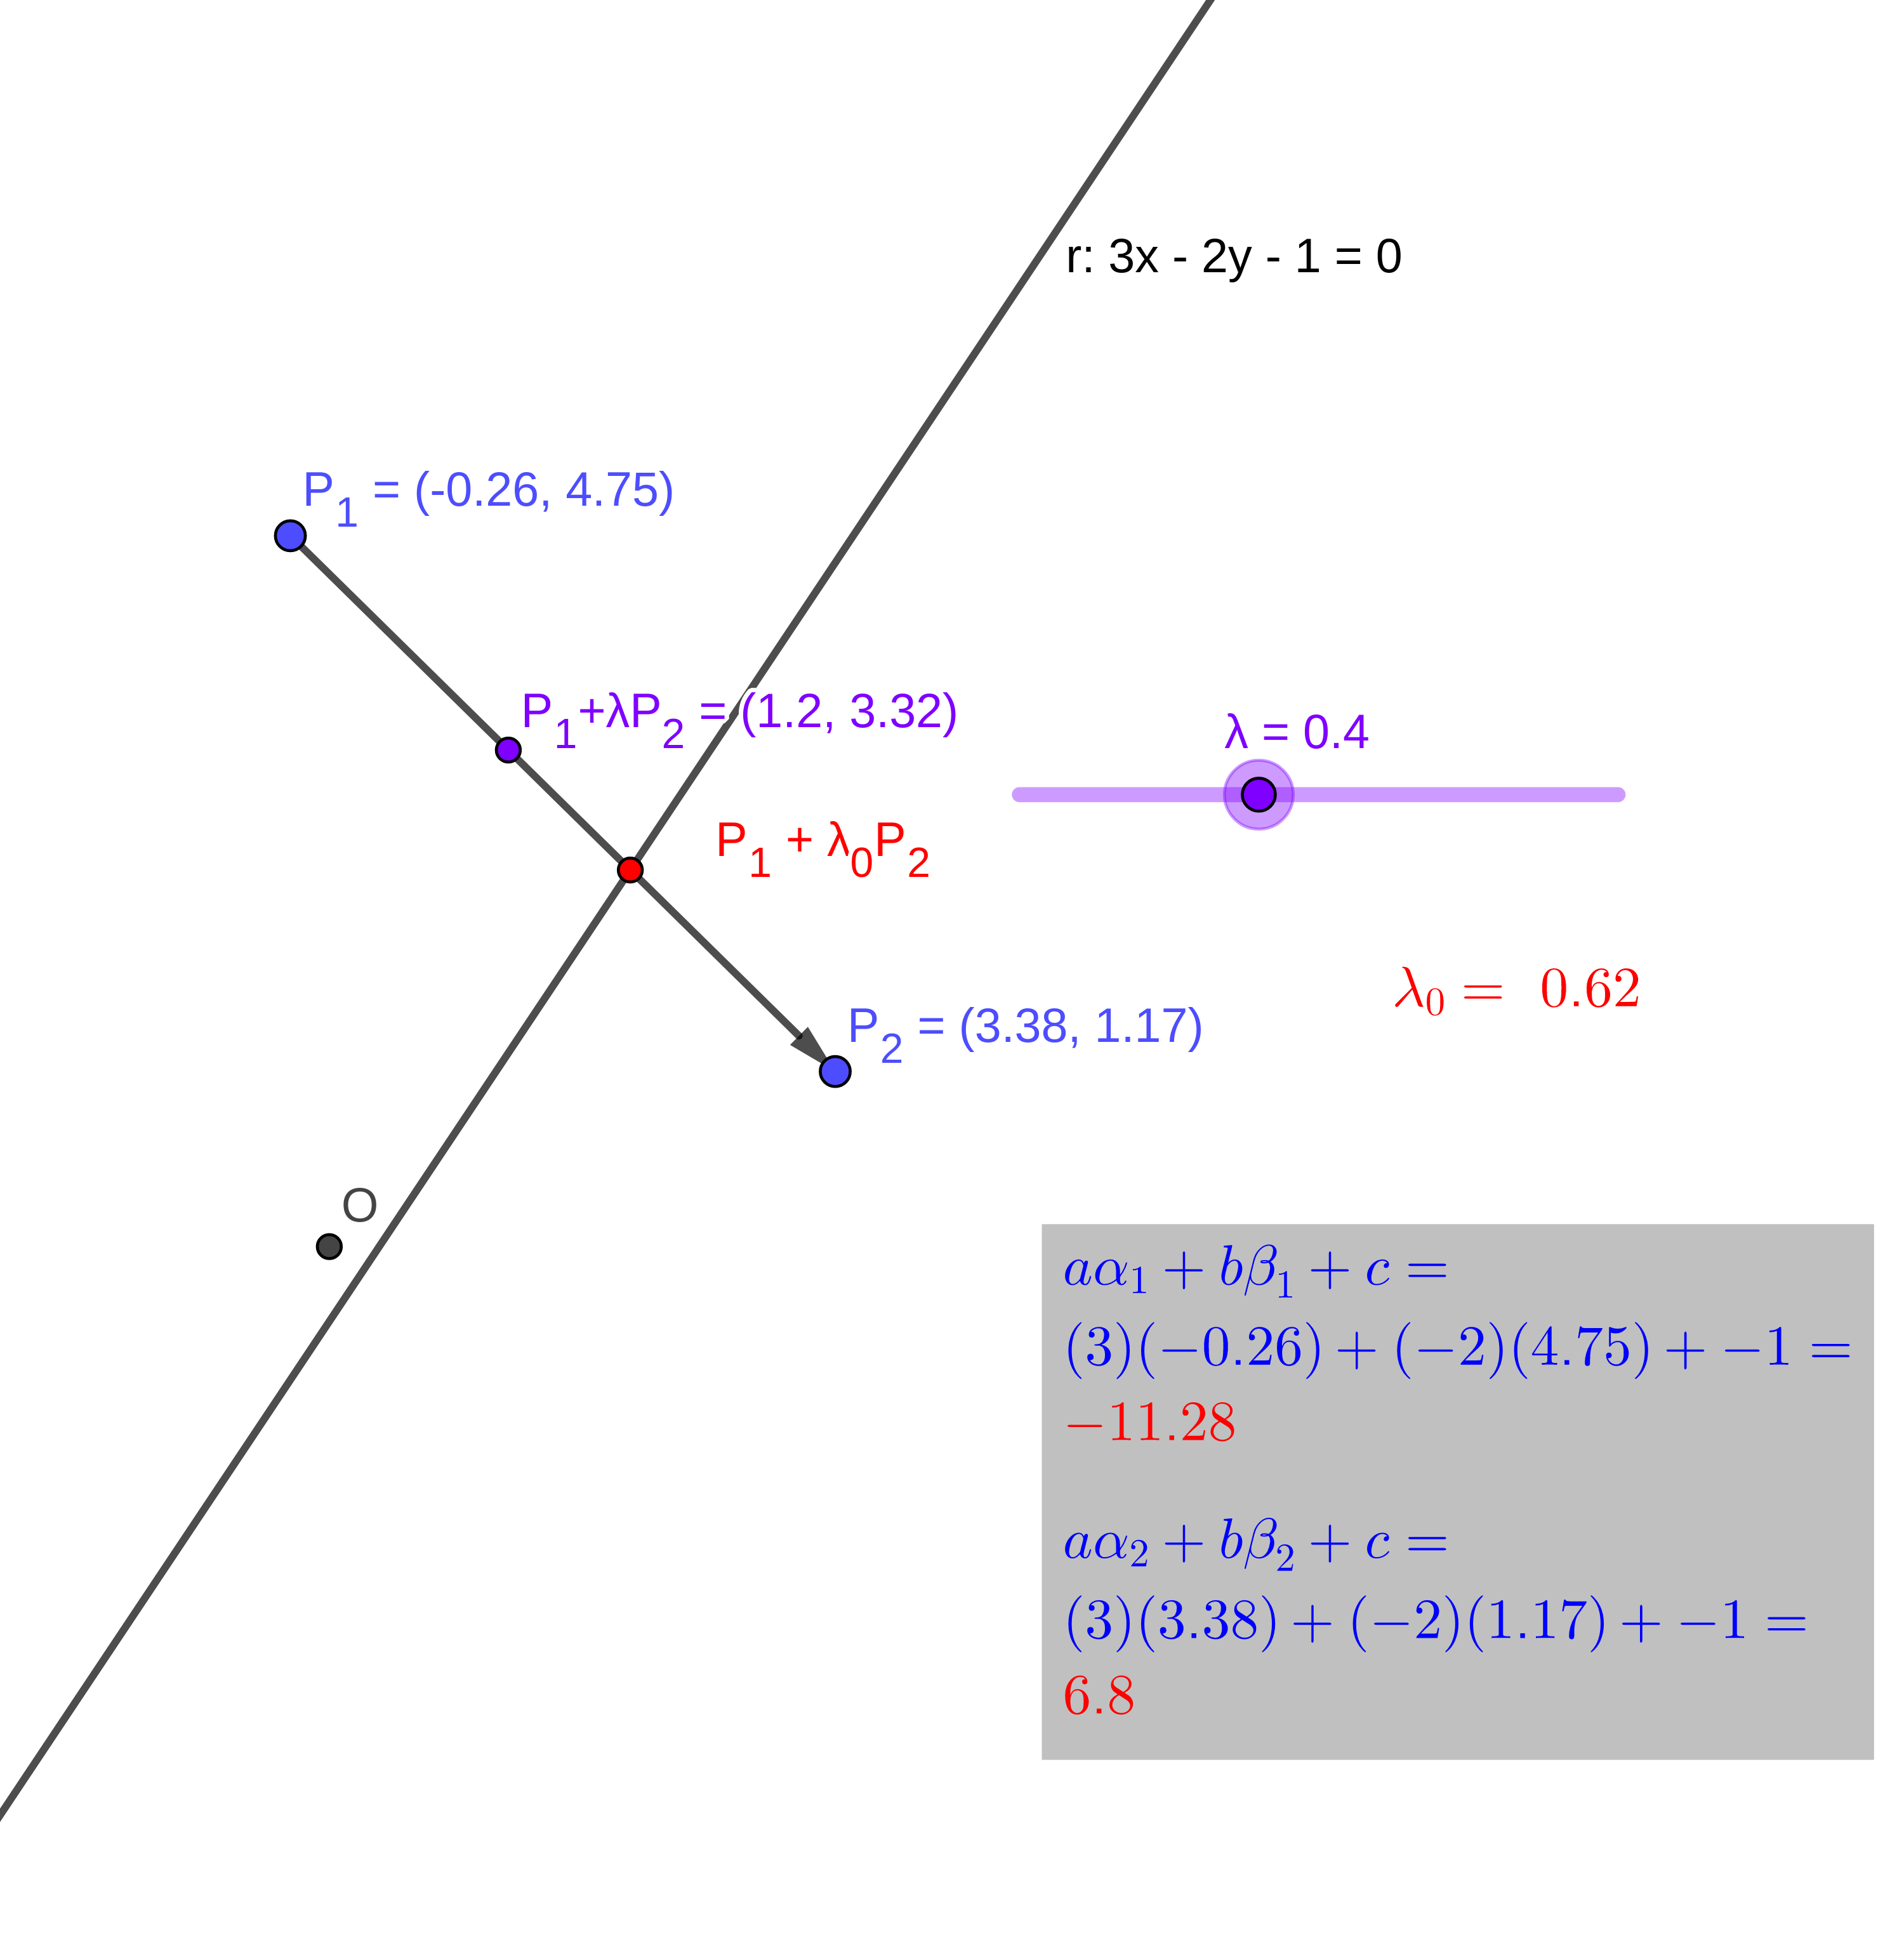
\includegraphics{Problema_01.png}
  \\
  Ejemplo del resultado obtenido.
  Imagen extra\'{\i}da del archivo Problema\_01(01).ggb
 \end{center}
 
\end{solucion}

